\documentclass[10pt,letterpaper]{article}
\usepackage[margin=0.8in]{geometry}
\usepackage[T1]{fontenc}
\usepackage{newtxtext,newtxmath}
\usepackage{microtype}
\usepackage{tikz}
\usetikzlibrary{arrows.meta}
\usepackage[font=small,labelfont=bf]{caption}
\usepackage[hidelinks]{hyperref}

\definecolor{plan}{HTML}{426684}
\definecolor{code}{HTML}{248582}
\definecolor{eval}{HTML}{B47C24}
\definecolor{alloc}{HTML}{80629D}
\definecolor{train}{HTML}{AF4545}
\definecolor{muted}{HTML}{68717C}
\setlength{\parindent}{1em}
\setlength{\parskip}{3pt}
\setlength{\textfloatsep}{11pt}
\setlength{\abovecaptionskip}{7pt}
\pagestyle{empty}
\hypersetup{pdftitle={Dependency-aware execution of the discovery loop}}

% One row represents a resource pool, not an individual worker. Coordinates
% illustrate ordering and overlap; they are not experimental timing data.
\newcommand{\activity}[5]{%
  \path[draw=#4!80!black,fill=#4!17,line width=0.45pt,rounded corners=1.4pt]
    (#1,{#3-0.17}) rectangle (#2,{#3+0.17});
  \node[font=\sffamily\scriptsize,text=#4!70!black,inner sep=0pt]
    at ({(#1+#2)/2},#3) {#5};}

\begin{document}
\subsection*{Dependency-aware execution of the discovery loop}

Each discovery step selects parents from an archive of evaluated candidates.
A frozen strategist proposes several strategies for each parent, and a
trainable coder generates strategy-conditioned programs in cross-prompt
batches. Parent chains are processed concurrently; within a chain, later
strategies can condition on earlier proposals. Each strategy first receives
a pilot batch. Once all pilot evaluations for a parent are available, a
strategy-level bandit assigns that parent's remaining rollout budget using
the observed outcomes and estimated opportunity for improvement. These
allocations form batches of phase-2 programs; the allocation calculation
does not require generating and evaluating one additional program at a time.
Pilot and phase-2 samples both contribute to coder training.

\begin{figure}[ht]
\centering
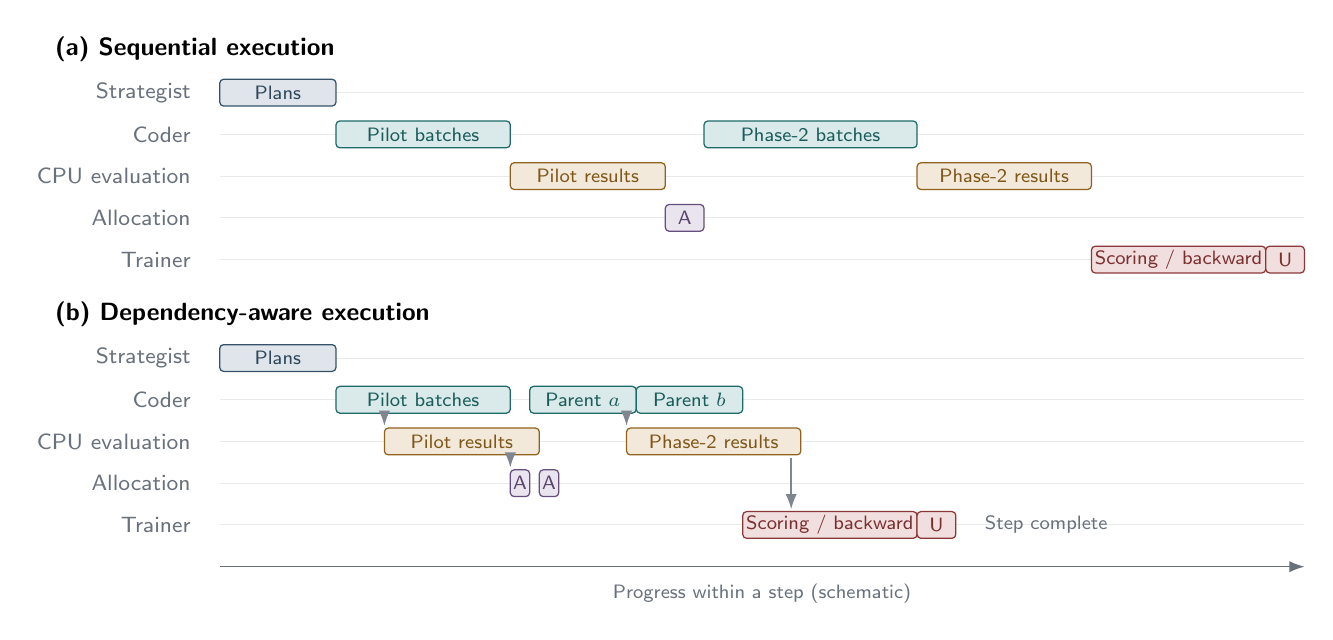
\begin{tikzpicture}[x=0.123cm,y=1cm,>=Latex,
    every node/.style={font=\sffamily\small},
    lane/.style={font=\sffamily\footnotesize,anchor=east,text=muted},
    flow/.style={->,draw=muted!85,line width=0.55pt}]

  \node[anchor=west,font=\sffamily\bfseries\small] at (-18,0.55)
    {(a) Sequential execution};
  \foreach \label/\y in {Strategist/0,Coder/-0.53,CPU evaluation/-1.06,Allocation/-1.59,Trainer/-2.12}{
    \node[lane] at (-2,\y) {\label};
    \draw[muted!15,line width=0.35pt] (0,\y) -- (112,\y);
  }
  \activity{0}{12}{0}{plan}{Plans}
  \activity{12}{30}{-0.53}{code}{Pilot batches}
  \activity{30}{46}{-1.06}{eval}{Pilot results}
  \activity{46}{50}{-1.59}{alloc}{A}
  \activity{50}{72}{-0.53}{code}{Phase-2 batches}
  \activity{72}{90}{-1.06}{eval}{Phase-2 results}
  \activity{90}{108}{-2.12}{train}{Scoring / backward}
  \activity{108}{112}{-2.12}{train}{U}

  \begin{scope}[yshift=-3.37cm]
    \node[anchor=west,font=\sffamily\bfseries\small] at (-18,0.55)
      {(b) Dependency-aware execution};
    \foreach \label/\y in {Strategist/0,Coder/-0.53,CPU evaluation/-1.06,Allocation/-1.59,Trainer/-2.12}{
      \node[lane] at (-2,\y) {\label};
      \draw[muted!15,line width=0.35pt] (0,\y) -- (112,\y);
    }
    \activity{0}{12}{0}{plan}{Plans}
    \activity{12}{30}{-0.53}{code}{Pilot batches}
    \activity{17}{33}{-1.06}{eval}{Pilot results}
    \activity{30}{32}{-1.59}{alloc}{A}
    \activity{33}{35}{-1.59}{alloc}{A}
    \activity{32}{43}{-0.53}{code}{Parent $a$}
    \activity{43}{54}{-0.53}{code}{Parent $b$}
    \activity{42}{60}{-1.06}{eval}{Phase-2 results}
    \activity{54}{72}{-2.12}{train}{Scoring / backward}
    \activity{72}{76}{-2.12}{train}{U}
    \draw[flow] (17,-0.72) -- (17,-0.86);
    \draw[flow] (30,-1.26) -- (30,-1.39);
    \draw[flow] (42,-0.72) -- (42,-0.86);
    \draw[flow] (59,-1.27) -- (59,-1.92);
    \node[anchor=west,font=\sffamily\scriptsize,text=muted]
      at (78,-2.12) {Step complete};
    \draw[->,draw=muted,line width=0.55pt] (0,-2.65) -- (112,-2.65);
    \node[font=\sffamily\scriptsize,text=muted,anchor=north]
      at (56,-2.74) {Progress within a step (schematic)};
  \end{scope}
\end{tikzpicture}
\caption{\textbf{Overlap execution, preserve dependencies.}
Sequential scheduling waits for each entire stage. The implemented schedule
evaluates completed programs during generation, allocates phase 2 when a
parent's pilot results are ready, and overlaps training with the remaining
evaluations. Parent $a$ and parent $b$ denote phase-2 batches;
A denotes allocation and U the final optimizer update.
Bar lengths are illustrative, not measured runtimes or a speedup claim.}
\label{fig:implementation-pipeline}
\end{figure}

Evaluation is driven by completion rather than by a global generation
barrier. As each completed program is returned by the generator, it is saved
and submitted to a CPU execution and verification pool. Evaluation therefore
overlaps subsequent rollout generation in both phases. A ready parent's
phase-2 work can be dispatched while other parents' pilots are still being
evaluated. The program's parent, strategy, prompt, generated tokens, and
evaluation outcome remain associated throughout the pipeline.

Once rollout generation and required policy scoring finish, the shared
GPUs transition to training without waiting for the entire CPU evaluation
queue to drain. Training inputs are prepared, and each reward-ready sample
enters the distributed work queue for SPO-RS loss evaluation and backward
computation. The historical normalization used to form its advantage is
held fixed for the step, so unrelated pending rewards need not delay this
work. All rollouts and training forwards use the same pre-update coder
policy. Gradients accumulate without changing model parameters; the optimizer
update is applied only after all required rewards and gradients are available
and the rollout artifacts have been saved. The strategist remains frozen.

The evaluated candidates update the search archive and parent--child tree.
The completed step saves the updated coder and search state for the next
iteration. When an LLM-based parent selector is enabled, its next-step
request can run during the remaining training work, using the newly
evaluated tree. Thus, concurrency removes avoidable waiting between
independent tasks without removing the data dependencies that define
allocation, training, or parent selection.

\end{document}
